%---------change this every homework
% place your email id between the braces so that your homework has a name
\def\yourname{Hamlet}
% -----------------------------------------------------
\def\homework{1} % 0 for solution, 1 for problem-set only
\def\duedate{February {\bf 19} at 5pm}
\def\duelocation{via \href{https://www.gradescope.com/courses/225474}{gradescope}}
\def\hnumber{4}
\def\prof{Andrew Drucker, Lorenzo Orecchia}
\def\course{\href{https://canvas.uchicago.edu/courses/33273}{CMSC 27200 - Winter 2021}}
%-------------------------------------

\documentclass[10pt]{article}
\usepackage[colorlinks,urlcolor=blue]{hyperref}
\usepackage[osf]{mathpazo}
\usepackage{amsmath,amsfonts,graphicx}
\usepackage{algpseudocode}
\usepackage{tikz}
\usepackage{latexsym}
\usepackage{subfig}
\usepackage{enumerate}
\usepackage{listings}
\usepackage{fullpage}
\usepackage{color}
\definecolor{mdb}{rgb}{0.3,0.02,0.02}
\definecolor{cit}{rgb}{0.05,0.2,0.45}
\markboth{\yourname}{\yourname}

\thispagestyle{empty}

\newenvironment{proof}{\par\noindent{\it Proof.}\hspace*{1em}}{$\Box$\bigskip}
\newcommand{\qed}{$\Box$}
\newcommand{\alg}[1]{\mathsf{#1}}
\newcommand{\handout}{
   \renewcommand{\thepage}{H\hnumber-\arabic{page}}
   \noindent
   \begin{center}
      \vbox{
    \hbox to \columnwidth {\sc{\course} --- \prof \hfill}
    \vspace{-2mm}
    \hbox to \columnwidth {\sc due \MakeLowercase{\duedate} \duelocation\hfill {\Huge\color{mdb}H\hnumber.\yourname}}
      }
   \end{center}
   \vspace*{2mm}
}
\newcommand{\solution}[1]{\medskip\noindent{\color{cit}\textbf{Solution:} #1}}

\newcommand{\bit}[1]{\{0,1\}^{ #1 }}
\newtheorem{problem}{\sc\color{cit}problem}
\newtheorem{lemma}{Lemma}
\newtheorem{theorem}{Theorem}
\newtheorem{definition}{Definition}
\newtheorem{claim}{Claim}


\begin{document}
\handout
\begin{itemize}
\item The assignment is due at Gradescope on {\bf Friday}, February 19 at 5pm.

\item You can either type your homework using LaTeX or scan your handwritten work. We will provide a LaTex template for each homework. If you writing by hand, please fill in the solutions in this template, inserting additional sheets as necessary. This will facilitate the grading.

\item You are permitted to discuss the problems with up to 2 other students in the class (per problem); however, {\em you must write up your own solutions, in your own words}. Each student is expected to independently make their own writeup of solutions, and provide clearly expressed mathematical arguments.

\item Consulting problem solutions on the web is not allowed.  Any sources used, including collaborators, textbooks other than the two listed on the syllabus, lecture notes from other courses, and learning material found on the web must be explicitly acknowledged.

\item {\em Show your work.} Answers without justification will be given little credit.
\end{itemize}

%%%%%%%%%%%%%%%%%%%%%%%%%%%%%%%%%%%%%%%%%%%
% PROBLEM 1
%%%%%%%%%%%%%%%%%%%%%%%%%%%%%%%%%%%%%%%%%%%
\newpage
\begin{problem}[Hopping Game with Rewards] ($35$ points)
\end{problem}
In a previous problem, we considered a hopping game where you can hop 1, 2, 3, or 4 spaces forward and spaces are marked either O or X (where O is safe and X is an obstacle which makes you lose the game.)

Now let's say that spaces have penalties and rewards. More precisely, each space $i$ has a value $v_i$ which can be the following
\begin{itemize}
\item $v_i = -\infty$: This space has an obstacle which makes you lose if you land on it.
\item $v_i < 0$: This space does not have an obstacle, but you pay a penality $v_i$ if you land on it.
\item $v_i = 0$: This space does not have an obstacle, incurs no penality, but also offers no reward.
\item $v_i > 0$: This space does not have an obstacle, and you receieve a reward of value $v_i$ for landing on it.
\end{itemize}

Design an algorithm running in time $O(n)$ to determine the largest amount of reward you can pick up while reaching the end (square $n$) from the beginning (square 0, assumed safe) in at most $n$ hops. Prove your algorithm's correctness and efficiency.

\solution{

\begin{algorithmic}
  \For {$v_i$, $i < n$}
    \If {there exists a nonnegative value $v_j$ within 4 spaces}
    \State Jump to $v_j$
    \Else {the next 4 spaces have a negative value}
    \State Jump to $v_j$ where $v_j = max\{v_{i+1} + v_{i+5}, v_{i+2} + v_{i+5}, v_{i+2} + v_{i+6}, v_{i+3} + v_{i+5}, v_{i+3} + v_{i+6}, v_{i+3} + v_{i+7}, v_{i+4} + v_{i+5}, v_{i+4} + v_{i+6}, v_{i+4} + v_{i+7}, v_{i+4} + v_{i+8}\}$
    \EndIf
  \EndFor
\end{algorithmic}

\paragraph{Proof of Runtime}

\paragraph{Proof of Correctness} This proof will be using a Dynamic Programming approach. 

\subparagraph{Family of Subproblems} Let our Input Array be $A[i] = {v_1, v_2, \ldots v_n}$ where $i \leq n$. Let our Output array be a subsequence of values that represent our jumps, each 
value of our subsequence is at max a distance of 4. Let $J \subseteq [n]$ and we want to maximize $V(J) = \sum V_j$ where $V(J)$ is the sum of all the values we jumped to. Now, 
we want to establish the k'th problem subfamily. Our subproblem will maintain the same goal as our problem but also $J \subseteq [k], k < n$ where J is "k-restricted". 

\subparagraph{Define Solutions} We will be using $OPT_k$ to define the solution for our subproblem. $Opt_n$ is our final solution. We can establish that our Base Case for both 
$Opt_k$, $Opt_n$ is $OPT_0 = v_0$ since we can assume we begin at space 0.

\subparagraph{Proof} We will now define $OPT_{k+1}$. We claim that for $1 < k < n$, $OPT_{k+1} = max\{OPT_k, v_{k+1} + OPT_l\}$ where $l$ is an index defined as $l = max\{j \leq k + 4, v(j) \leq v(k)\}$. $l$ 
is an index smaller k at a maximum distance of 4. We want to show that 1: $Opt_{k+1} \geq OPT_k$ and 2: $OPT_{k+1} \geq v_{k+1} + OPT_l$.

\subparagraph{1} $OPT_{k+1} \geq OPT_k$. We know $V(J) = OPT_k$. Since $J$ is k-restricted we know that $J$ is also k+1 restricted because the first k values jumped to are a subset of the first
k+1 values jumped to. Therefore we know $OPT_{k+1} \geq V(J)$.

\subparagraph{2} $OPT_{k+1} \geq v_{k+1} + OPT_l$. Let $J'$ be l-restricted then $V(J') = OPT_l$ where we know $l \neq k, J' \neq J$. Then $V_{k+1} + OPT_l = \{k+1\} \cup J' = J''$. $J''$ is 
k+! restricted by definition because it goes up to and included k+1. We know this is feasible by definition of l, $v_l$ is within hopping distance of $v_{k+1}$. Thus, we know 
$OPT_{k+1} \geq V(J')$.

\subparagraph{Finishing Proof} We want to show $OPT_{k+1} \geq max\{OPT_k, v_{k+1} + OPT_l\}$. Let $J$ be k+1 restricted and $V(J) = OPT_{k+1}$ we ask ourselves, is $(k+1) \in J$? If no then J is k restricted which 
we already know as $V(J) \geq OPT_k$. If Yes, we know $J = \{k+1\} \cup J*$. We know that $J*$ must be smaller than J and is therefore l-restricted. We know that $J$ is feasible because by definition value l is within hopping distance. So, 
$V(J) \geq V_{k+1} + OPT_l$. 

}

\newpage
\medskip\noindent{\color{cit} Extra Space for your solution}


%%%%%%%%%%%%%%%%%%%%%%%%%%%%%%%%%%%%%%%%%%%
% PROBLEM 2
%%%%%%%%%%%%%%%%%%%%%%%%%%%%%%%%%%%%%%%%%%%
\newpage
\begin{problem}[Shortest Paths][10+20 = 30 points]
\end{problem}

\begin{enumerate}[a.]
\item Assume you were to run Dijkstra's shortest paths algorithm starting from node $a$. Find one node where the algorithm finds incorrect distance due to the negative edge weights in the graph. Please specify the (incorrect) distance that Dijkstra's outputs and the true distance between $a$ and the node.

\begin{center}
%\includegraphics[scale=0.45]{Bellman_Ford_graph.pdf}
\end{center}

\item Find the shortest paths from each node to $t$ in the same graph using the Bellman-Ford algorithm. Show your work by writing out the dynamic programming table, as in Figure 6.23 on page 294 of the textbook. Please follow the same format as in that figure or you may be deducted points. At the end, please state the distance of each node from $t$.
\end{enumerate}
\solution{

\section{A}

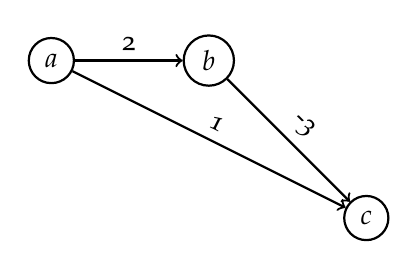
\begin{tikzpicture}[node distance={20mm}, thick, main/.style = {draw, circle}] 
  \node[main] (1) {$a$};
  \node[main] (2) [right of=1] {$b$};
  \node[main] (3) [right of=1, below of=2] {$c$};
  \draw[->] (1) -- node[midway, above, sloped] {2} (2);
  \draw[->] (1) -- node[midway, above, sloped] {1} (3);
  \draw[->] (2) -- node[midway, above, sloped] {-3} (3);


\end{tikzpicture} 

\paragraph{Explanation} This problem illustrates why Dijkstra's algorithm does not work with negative edges because Dijkstra's algorithm assumes distances explored are always correct.
As a greedy algorithm, Dijkstra's establishes an explored set of nodes and assumes that distances already calculated, and vertices already part of the explored set, are shortest giving no room for future paths to be shorter. 
In fact, when given a graph of nonnegative values Dijkstra's algorithm is correct to assume that once calculated paths are always shortest because positive values always increase sums. However, when negative values are introduced
vertices within the explored set can have new shorter paths. Using our example, Dijkstra's algorithm would say that the shortest path from node A to C to along edge of length 1. However, this distance is incorrect because taking 
the path from A to B then to C would give a total distance of $-1$ which is shorter. Dijkstra's does not include $A \rightarrow B \rightarrow C$ as a path because A can get to C from one edge, and once C is explored there can be no change. 


\section{B}

\begin{tabular}{c|c|c|c|c}
    Successor & & 0 & 1 & 2 \\
  & c & 0 & 0 & 0 \\
  b & a & $\infty$ & 1 & $-1$ \\
  c & b & $\infty$ & $-3$ & $-3$  \\
\end{tabular}

\paragraph{Explanation} Using our example from part A, our graph does not contain any negative cycles and we can therefore use the Bellman-Ford algorithm. Using the algorithm we can draw our correct
shortet paths: starting from the value that gives us the minimum distance to $c$ we can trace the successors back to $c$. Thus, since our minimum distance at the end of 3 iterations is $-1$ we can start at vertex $a$,
travel to its successor $b$ then travel to its successor $c$. We know the total distance is $-1$ and the cheapest. A step by step explanation would detail as follows:

\subparagraph{} We work down the table. Since $c$ is our terminal vertex therefore for $i = 0, 1, 2$ the distance is 0. For both $a$ and $b$ at $i = 0$ they have a chapest distance of $\infty$. 
For $i = 1$ $a$ has to edges to work with. Edge $ac$ has a value of 1 and a total of $1 + \infty$. Edge $ab$ has a value of 2 and a total of $2 + \infty$. We take the minimum of these two values and for $i = 1$ the cheapest distance
to c is edge $ac$ with a distance of 1. We update the successor for a which is c. Next, for $i = 1$ vertex b only has one edge going outwards with a value of $-3$ and since $-3 + \infty$ is less than the 
previous value of $\infty$ we update the table with $b$ having a total distance of $-3$. The successor of $b$ is $c$. Next we can move onto $i = 2$. For $a$ we look at edge $ab$ with a value of $2$ which leads to vertex $b$ which has a value of $-3$. 
$2 + -3 = -1$ which is less than the previous value of $1$ for $a$. Therefore, we update the table for $a$ with a cheapest distance of $-1$ when $i = 2$ and update the successor from $c$ to $b$. For $b$ it only has
one outward edge so it remains at $-3$. Thus our table is complete and we follow the path from $a \Rightarrow b \Rightarrow c$ with a total distance of $-1$.   


}

\newpage
\medskip\noindent{\color{cit} Extra Space for your solution}

%%%%%%%%%%%%%%%%%%%%%%%%%%%%%%%%%%%%%%%%%%%
% PROBLEM 3
%%%%%%%%%%%%%%%%%%%%%%%%%%%%%%%%%%%%%%%%%%%
\newpage
\begin{problem}[Mobile Networks][35 points]
\end{problem}
Do exercise 14 in Kleinberg-Tardos, Chapter 6. For both subproblems, prove that your algorithm is correct and runs in polynomial time.

\solution{

\begin{algorithmic}
  \State Let array $A[0, 1, \ldots n]$ be our array of indexes 
  \State Set $A[0] = 0$
  \For {All paths $P_i, P_j$ where $i \leq j$}
  \State Find shortest number of edges using Breadth First Search
  \EndFor
  \For {$j = 1,2, \ldots n$}
  \State Compute $A[j] = OPT(j)$
  \EndFor
  \State Return $A[n]$ \\

  \State FindPaths(j)
  \If {$j = 0$}
  \State output nothing
  \Else
  \State Find $i = min(cost_{ij} + K + A[i-1])$, output paths $P_i, P_{i + 1}, \ldots P_j$ and FindPaths($i-1$). 
  \EndIf
\end{algorithmic}

\paragraph{Proof of Runtime} Since we are computing the shortest path for each Graph $G_i$ using Breadth First Search we know that the time complexity is at least that
of BFS, $O(m+n)$ where if $G_i = (V, E_i)$ then $n = |V|, m = |E_i|$. To fin dthe shortest path we must loop twice over all n paths, for each $P_i$ for $G_i$ we must 
compares edges against all other paths giving us a time complexity of $O(n^2)$. This means that our runtime for an optimal solution
using BFS is $O((m+n)n^2)$ which is polynomial time. 

\paragraph{Proof of Correctness} We will prove this algorithm using Dynamic Programming. Let's re-establish out input. We have a set of Graphs
with a set of vertices $(V)$ and a changing set of Edges $E_i = (E_1, E_2, \ldots E_n)$ where $1 \leq i \leq n$. We know that for a given point in time, $G_i = (V, E_i)$. Our goal for this proof is to 
find the shortest path in each $G_i$. First, we want to define our solutions. Let $OPT_i$ be the optimal solution for graph $G_i$ where $P_i$ is the shortest path from a source vertex $s$ to a terminal vertex $t$. We know 
$P_i$ is feasible because we are given the assumption that for any $G_i$ the graph is connected. Therefore, we know there exists a path $P_i$ between $s$ and $t$. Let $l(P_i)$ denote the length of the shortest path. Let 
$cost_{ij} = cost(P_i, P_{i+1}, \ldots P_j) = \sum_{i = 1}^{b} l(P_i) + K*changes(P_i, P_{i+1}, \ldots P_j)$. With this definition we can define the value $OPT(n)$ as $OPT(n) = cost_{ij} + K + OPT(i-1)$. Effectively, we are breaking up 
the sectiosn of time in which the Graph evolves by the paths of each Graph. Our goal is to find the shortest path that also contains the smallest amount of change between graphs therefore we can choose one segment of Graphs, $G_i to G_j$
find the shortest path with the minimum cost for those graphs and then recurse over the Graphs $G_1$ to $G_{i-1}$. At this point we can establish that for $G_0$, $OPT(0) = G_0$ and this graph can be treated as our base case. 

\subparagraph{Family of subproblems} After defining our solutions, we want to define our family of subproblems. For the subproblem $P_1, P_2, \ldots P_j$, we must find the best segment of paths $P_i, \ldots P_j$ in $OPT_j$. 
To find the shortest path along with the least amount of change we can define $OPT_j$ as $OPT_j = min_{1 \leq i \leq j} (cost_{ij} + K + OPT(i-1))$. Thus, for any subproblem we want to find the shortest path with minimum changes 
between $P_i$ and $P_j$ and we can recurse over $OPT(i-1)$. Thus using these definitions our recurrense relation can be defined as $OPT_j \geq min_{1 \leq i \leq j} (cost_{ij} + K + OPT(i-1))$. 

\subparagraph{Proof of Recurrence Relation} Since our optimal solution is $OPT_n$, we want to build up towards $OPT_n$ using $OPT_j$, therefore we want to define and prove $OPT_{j+1}$. We can define $OPT_{j+1}$ as 
$OPT_{j+1} \geq min\{OPT_j, l(P_{j+1}) + min_{1 \leq i \leq j} (cost_{j, j+1} + K + OPT(j))$. We want to show that $OPT_{j+1}$ is at most either $OPT_j$ or $l(P_{j+1}) + min_{1 \leq i \leq j} (cost_{j, j+1} + K + OPT(j)$. First,
we want to show $OPT_{j+1} \geq OPT_j$. We know that $OPT_j = P_j$ where $P_j$ is the shortest path with minimum change. Well, by definition $OPT_{j+1} = min_{1 \leq i \leq j} (cost_{j, j+1} + K + OPT(j)$ which includes $OPT_j$. By difference of $cost_{j,j+1} + K$, we know that
$OPT_{j+1} \geq OPT_j$. Next, we want to show, $OPT_{j+1} \geq l(P_{j+1}) + min_{1 \leq i \leq j} (cost_{i, j} + K + OPT(i-1)$. We know that adding $l(P_{j+1})$ adds to the cost of the Paths, which we can denote as $cost_{i,j} + cost_{j, j+1}$. We must consider 
the constant K with each cost, we must still recurse over the segments prior to $OPT(i-1)$ which can all be defined as: $OPT_{j+1} \geq min_{1 \leq i \leq j} (cost_{j, j+1} + K + cost_{i,j} + K + OPT(i-1))$. However, $OPT_j = cost_{i,j} + K + OPT(i-1)$ so we can \
further define $OPT_{j+1} \geq min_{1 \leq i \leq j} (cost_{j, j+1} + K + OPT_j)$. This is feasible because adding the length of $P_{j+1}$ maintains the graph as connected as per our assumption.  




}




\newpage
\medskip\noindent{\color{cit} Extra Space for your solution}


\end{document}
